\documentclass[11pt, a4paper]{article}

\usepackage[a4paper, margin=2.5cm]{geometry}

\usepackage{amsmath}
\usepackage{booktabs}
\usepackage{tabularx}
\usepackage{enumitem}
\usepackage{graphicx}
\usepackage[export]{adjustbox}
\usepackage{xcolor}
\usepackage{hyperref}
\usepackage{parskip}
\usepackage{amssymb}
\usepackage{float}

\title{\textbf{Supermarket Database --- Design Specification}}
\author{}
\date{}

\begin{document}

\maketitle

\begin{figure}[H]
    \centering
    
    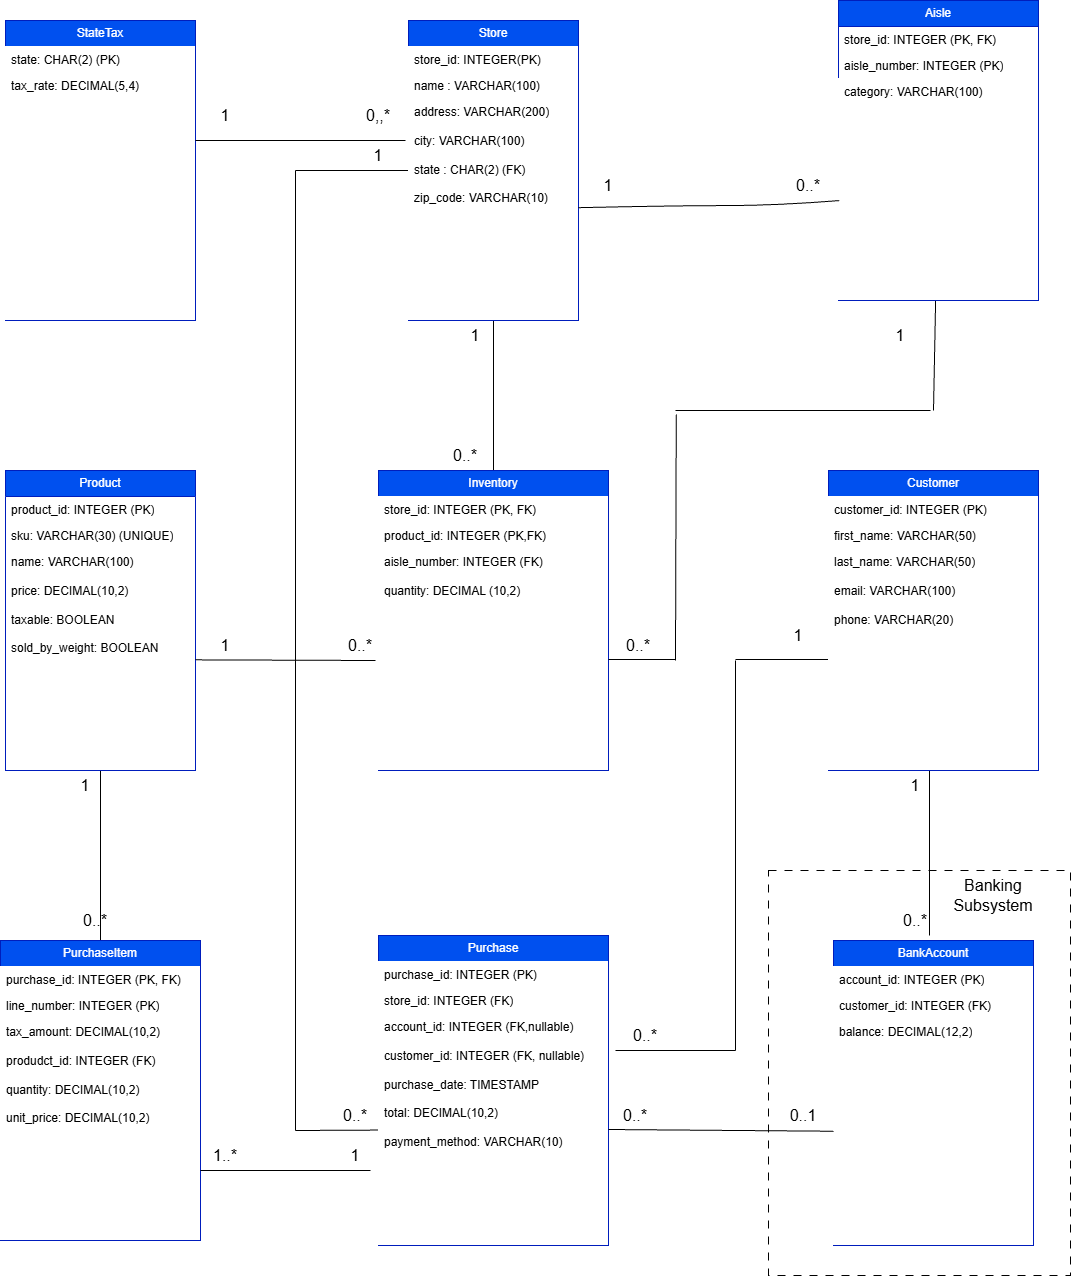
\includegraphics[width=0.85\textwidth, frame]{er-diagram_png.png}
       
    \caption{Supermarket Database ER Model Draft}
    \label{fig:er_model}
\end{figure}

\begin{figure}[H]
    \centering
    
    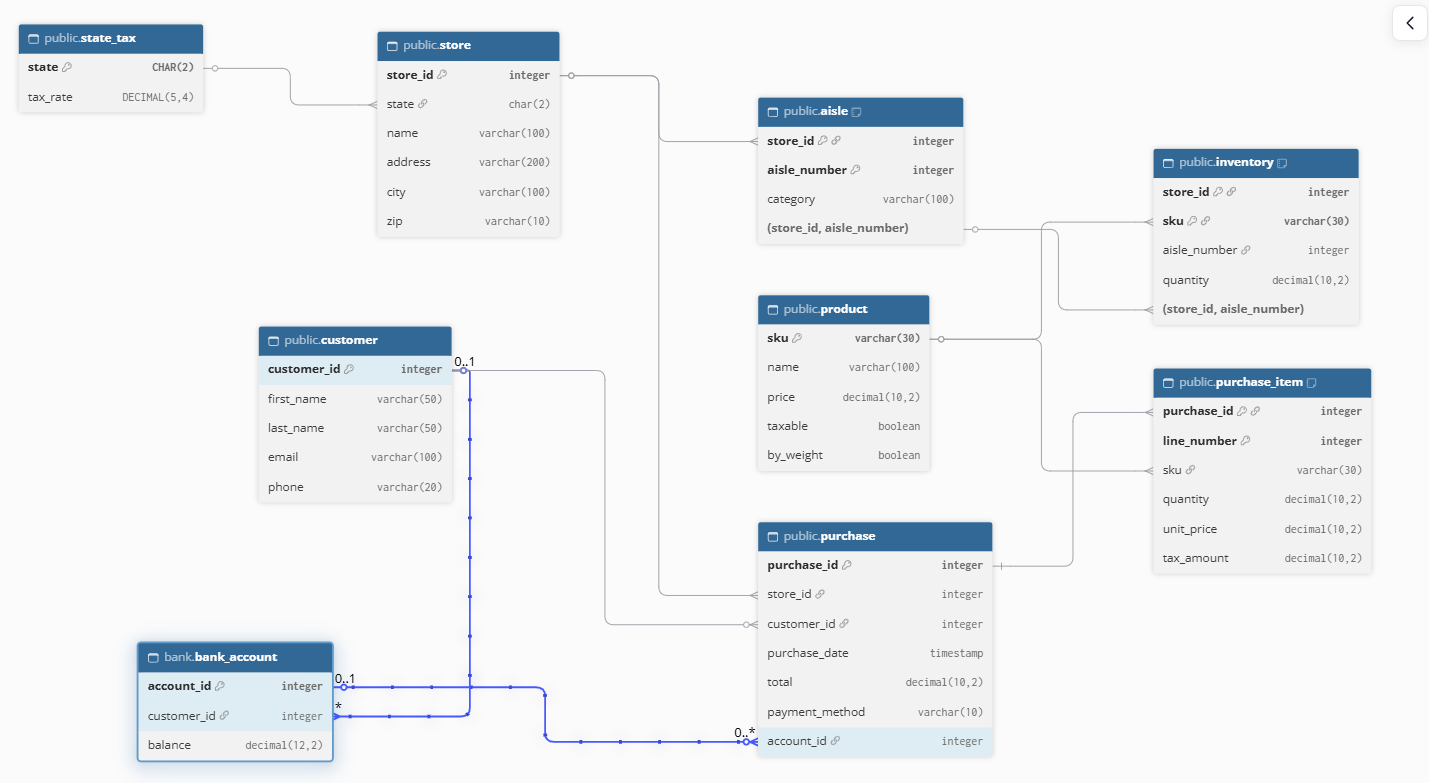
\includegraphics[width=0.85\textwidth, frame]{er-diagram2.png}
       
    \caption{Preliminary ERD Locked In Before Phase 1}
    \label{fig:er_model}
\end{figure}

\section{Project Overview}
This project implements a relational database for a supermarket chain using PostgreSQL.

The system will simulate supermarket checkout operations, including product purchases, inventory management, sales tax calculations, receipt generation, and payment processing.

The database will support a JavaScript web application with customer-facing checkout operations and back-office reporting.

\section{Database Requirements}
The database must support:
\begin{itemize}[leftmargin=1.5em, itemsep=2pt]
    \item Multiple supermarket locations across at least four states.
    \item At least 100 stores, each containing 20--40 aisles.
    \item Products identified by SKU.
    \item Store-specific inventory quantities.
    \item Products sold by unit or weight.
    \item State-dependent sales taxes, including tax-exempt products.
    \item Cash and card payments.
    \item Purchase receipts containing individual items and totals.
    \item Card payments that update a separate bank account table.
    \item SQL transactions that modify multiple tables atomically.
    \item Reporting queries involving joins and aggregations.
\end{itemize}

\section{Preliminary Database Entities}
\begin{table}[htbp]
    \centering
    \begin{tabularx}{\textwidth}{l X}
        \toprule
        \textbf{Entity} & \textbf{Description} \\
        \midrule
        Store        & Physical supermarket location \\
        Product      & Product catalog containing SKU, price, and tax status \\
        Inventory    & Stock quantities for products at individual stores \\
        Customer     & Customer identification and associated information \\
        BankAccount  & Account balances used for simulated card payments \\
        Purchase     & Checkout transaction and receipt summary \\
        PurchaseItem & Individual receipt line items \\
        StateTax     & State-level sales tax rates \\
        \bottomrule
    \end{tabularx}
    \caption{Core Preliminary Database Entities}
    \label{tab:entities}
\end{table}

Additional entities, such as \texttt{Aisle}, may be introduced during ER refinement.

\section{Preliminary Relationships}
\begin{itemize}[leftmargin=1.5em, itemsep=2pt]
    \item One Store has many Inventory records.
    \item One Product can appear in many Inventory records.
    \item One Store processes many Purchases.
    \item One Customer can make many Purchases.
    \item One Purchase contains many PurchaseItems.
    \item One Product can appear in many PurchaseItems.
    \item One Customer may have an associated BankAccount.
    \item One StateTax record may apply to multiple Stores.
\end{itemize}

\section{Primary and Foreign Keys}
The schema will use surrogate primary keys for major business entities.

Inventory will use a composite primary key:
\begin{center}
    \texttt{(store\_id, product\_id)}
\end{center}

PurchaseItem will use a composite primary key:
\begin{center}
    \texttt{(purchase\_id, line\_number)}
\end{center}

Foreign keys will enforce referential integrity across all related tables.

\section{Transaction Processing}
The primary database transaction simulates supermarket checkout. Operations include:
\begin{enumerate}[leftmargin=2.5em, itemsep=2pt]
    \item Validate the selected products and quantities.
    \item Verify sufficient inventory.
    \item Calculate the purchase total, including applicable taxes.
    \item Verify sufficient funds for card payments.
    \item Insert the purchase record.
    \item Insert individual purchase items.
    \item Reduce inventory quantities.
    \item Deduct the payment amount from the bank account when paying by card.
    \item Commit all changes together.
\end{enumerate}

If any operation fails, the transaction must roll back.

\section{Normalization}
The database will target Third Normal Form (3NF), with Boyce-Codd Normal Form (BCNF) considered where appropriate.

Product information, store information, inventory, customer information, and purchase records will be stored separately to reduce redundancy and update anomalies.

Receipt line items will preserve historical sale prices, even if current product prices change.

\section{Planned SQL Reports}
The initial application will support at least three JOIN-based reporting queries:
\begin{enumerate}[leftmargin=1.5em, itemsep=2pt]
    \item Sales totals by store.
    \item Product sales quantities and revenue.
    \item Customer purchase history with receipt totals.
\end{enumerate}

\section{Development Status}

\subsection{Phase 1: Preliminary Implementation}

\textbf{Status:} Design in progress

\textbf{Rubric Requirements:} Should have a preliminary ER model covering the minimum attributes listed above, at
least five SQL tables. Payment with card must be recorded on a bank account table, subtracting
the amount from the balance. You should develop a basic web app functionality sending SQL
to the DBMS: at least one transaction code block and at least 3 insightful queries, web app
working locally. The transaction must update at least two tables (one of them should be the
bank account). All queries should involve joins, which assumes your database ER model is
normalized.

The ER model should include the most detailed table for each target application: (1) detail
cellphone calls (duration), data usage (MBs) and total minutes/data and amount to pay. (2)
Each item in the receipt (price, quantity or weight) and total amount to pay. Phase 1 will be
PASS/FAIL. A team receiving FAIL cannot submit Phase 2.

The preliminary schema and relationships are subject to revision during ER modeling and normalization.

\renewcommand{\arraystretch}{1.5}
\begin{tabularx}{\textwidth}{@{} c X l @{}}
    \toprule
    \textbf{Status} & \textbf{Task Requirement} & \textbf{Completed By} \\
    \midrule
    \multicolumn{3}{@{}l}{\textbf{Delegation and Architecture}} \\
    \midrule
        $\blacksquare$ & UML ER Draft & Mark \\
        $\square$ & Audit \& finalize preliminary model & TBD \\
        $\square$ & Lock in the schema (exact table names, column names, data types) & TBD \\

    \midrule
    \multicolumn{3}{@{}l}{\textbf{Database and SQL Build}} \\
    \midrule
        $\square$ & Initialize database locally & TBD \\
        $\square$ & Write DDL CREATE TABLE scripts with primary/foreign keys & TBD \\
        $\square$ & Write INSERT scripts for dummy data & TBD \\
        $\square$ & Write transaction block updating two tables concurrently & TBD \\
        $\square$ & Write reporting queries using JOIN operations & TBD \\

    \midrule
    \multicolumn{3}{@{}l}{\textbf{Backend Logic}} \\
    \midrule
        $\square$ & Configure local database connection & TBD \\
        $\square$ & Create routes for frontend to call & TBD \\
        $\square$ & Test endpoints to verify DB access & TBD \\

    \midrule
    \multicolumn{3}{@{}l}{\textbf{Frontend GUI Build}} \\
    \midrule
        $\square$ & Build basic HTML skeleton with required forms and buttons & TBD \\
        $\square$ & Write calls to backend & TBD \\
        $\square$ & Implement buttons to drop/create/insert & TBD \\
        $\square$ & Implement view function & TBD \\
        $\square$ & Implement simulation button for concurrent transaction & TBD \\

    \midrule
    \multicolumn{3}{@{}l}{\textbf{Phase 1 Validation}} \\
    \midrule
        $\square$ & End-to-end test & TBD \\
        $\square$ & Force OLTP error to verify error handling & TBD \\
        $\square$ & Verify Phase 1 rubric requirements & TBD \\
    \bottomrule
\end{tabularx}



\subsection{Phase 2: Completed Web-App}

\textbf{Status:} Not Started

\textbf{Rubric Requirements:} a fully working web app, with a polished DB model, well-designed ER model complying
with ER-to-relational mapping, with all tables updated with transactions (no isolated INSERT
or UPDATE). The project report PDF will be submitted 1 day after the web app is submitted
(to give time for text polishing, but no changes allowed in source code).

\renewcommand{\arraystretch}{1.5}
\begin{tabularx}{\textwidth}{@{} c X l @{}}
    \toprule
    \textbf{Status} & \textbf{Task Requirement} & \textbf{Completed By} \\
    \midrule
    \multicolumn{3}{@{}l}{\textbf{Database \& Schema}} \\
    \midrule
        $\square$ & Normalize to 3NF/BCNF & TBD \\
        $\square$ & Build tables for store, state, aisle, product, and tax requirements & TBD \\
        $\square$ & Lookup tables with minimum 10 rows & TBD \\

    \midrule
    \multicolumn{3}{@{}l}{\textbf{Backend}} \\
    \midrule
        $\square$ & Back office reporting for money totals & TBD \\
        $\square$ & .sql files & TBD \\

    \midrule
    \multicolumn{3}{@{}l}{\textbf{Frontend}} \\
    \midrule
        $\square$ & Automate random selection, compute, and process & TBD \\
        $\square$ & OLTP error and dangerous display messages & TBD \\

    \midrule
    \bottomrule
\end{tabularx}

\subsection{Phase 3: Documentation}

\textbf{Status:} Not Started

\textbf{Requirements:} 

\begin{itemize}
    \item \textbf{Concurrency Testing:} Ensure compatibilty across multiple browsers and concurrent requests
    \item  \textbf{PDF:} call it ”teamXY.pdf” where XY is your team id (01,02,..,21,..30). Report in PDF format
        including ER diagrams, written summary of web app including SQL for transaction and SQL
        for a few important queries (i.e. the most importan tables), and http link to demo video. Your
        report should include a list of web references at the end, including websites you chose as reference
        to build your app.
    \item \textbf{Source Files:} verify all source code, diagram files and any useful document you got from the Internet.
        Source code and web app originality: It is expected all source code, databases and GUI will be
        different even if some source code, some tables, and website ideas are obtained from the Internet
    \item \textbf{Video:} 8 minutes max - stored in some public website (youtube, dropbox, Google drive, etc).
        No password please, long URL OK, make sure it opens by anyone in one click. Format: mp4,
        viewable on any browser. Do not upload video files to our servers as it takes too much space
        and this violates UH IT policies.
        You should record a video, covering both DB model, important SQL (transaction code block
        and a few queries) and showing the finished web application in Phase 2. We will have a Teams
        session where all teams, TAs and the professor will watch it. Format: MP4.
\end{itemize}

\end{document}